% subject: コンピュータサイエンス第一期末試験(雛形)
% date:    16/11/2
% LaTeX2e: Japanese

\documentclass[12pt]{article}
\pagestyle{empty}
\usepackage{ascmac}
\usepackage[dvips]{epsfig}

% local.mac

%%% STYLE PARAM.s (for A4) %%%
\textwidth=16cm
\textheight=240mm

\topmargin=0mm
\headsep=0cm
\headheight=0cm
\oddsidemargin=0cm
\evensidemargin=0cm
\marginparwidth=0cm

\footnotesep=15pt
%\footheight=1.5cm
%\footskip=1.5cm

\itemsep=0.1pt
\parindent=11pt

\def\baselinestretch{1.15}

%%% LOCAL MACRO DEF.s %%%

\newcommand{\OMIT}[1]{}

% Print control (skips)
%\newcommand{\bigskip}{\vskip12pt}
%\newcommand{\medskip}{\vskip6pt}
%\newcommand{\smallskip}{\vskip3pt}
\newcommand{\paragraphskip}{\vskip\topsep}

% Itemization, etc
\newcommand{\nitem}[1]{%
\par\noindent\hangindent20pt%
\hskip20pt\llap{#1~}}
\newcommand{\nnitem}[1]{%
\par\noindent\hangindent30pt%
\hskip30pt\llap{#1~}}

\begin{document}
\noindent
\hfill{\small 16.Nov.2016}

\noindent
\hfil
{\large\bf
コンピュータサイエンス第1\textemdash 期末試験 CS-4b\textemdash}
\hfil

\paragraphskip\noindent
※答案用紙は各問ごとに 1 枚使用して書くこと.\\
※答案用紙には各枚ごとに学籍番号と氏名を書くこと.

\paragraphskip
\nitem{\bf 問1.}(配点 15 点)\\
2 つのチーム(a チームと b チーム)が,
毎回 0 点から 4 点までを獲得できるゲームを 7 ラウンド行った.
その結果が配列 {\tt a}, {\tt b} に格納されており,
高い得点から見て,
高い得点をより多くの回数得たチームを勝ちとなる.
たとえば,
%
\[
\begin{array}{l}
{\tt a}~=~{\tt[1,3,3,3,4,3,1]}\\
{\tt b}~=~{\tt[2,2,2,3,3,3,4]}
\end{array}
\qquad
\mbox{--- ($\ast$)}
\]
%
だったとすると,得点 4 を得た回数が同じなので,
次に高い得点 3 を得た回数が,より多い a チームが勝ちである.
このようなゲームのために,
得点の得た回数を比較するプログラムを言語 Ruby で以下のように作った.
このプログラムについて以下の問いに答えよ.
(プログラムは配列 {\tt a}, {\tt b} の値が
格納されたところから書かれている.
また,問いを明確にするため,
途中まで左に行の番号をつけてあるが,
実際のプログラムには含まれないものとする.)

\begin{verbatim}
    0    配列 a, b に得点が格納されているものとする
    1    ca = Array.new(5,0)
    2    cb = Array.new(5,0)
    3    for  i  in  0..6
    4       ca[ a[i] ] = ca[ a[i] ] + 1
    5       cb[ b[i] ] = cb[ b[i] ] + 1
    6    end
    7    t = 4
         stop = 0
         while t >= 0  && stop == 0
            if ca[ t ] != cb[ t ]
               stop = 1
            end
            t = t - 1
         end
         if stop == 1
           (A) 
         else
           (B)
         end
\end{verbatim}

\nitem{(1)}
配列 {\tt a}, {\tt b} の値が ($\ast$) だったとする.
この時,
このプログラムを実行して 7 行目まで計算が進んだときに,
配列 {\tt ca}, {\tt cb} の値がどうなっているかを示せ.

\nitem{(2)}
試合の結果が引き分けだと断定するのは,
このプログラムの (A), (B) のどちらに進んだ場合だろうか?

\nitem{(3)}
上記の問いの答えと逆に進んだ場合には,
チーム a と b のどちらかが勝ちのはずである.
それでは
勝敗を決めるには,
そこでどのような計算をすればよいだろうか?
具体的には,
次のようなプログラムで勝敗を決めるとすると,
(C) の部分は,どのような条件式になるだろうか?
(答えは Ruby の文法に正確に従っていなくてもよい.)

\begin{verbatim}
            if (C)
               a が勝ちと答える
            else
               b が勝ちと答える
            end
\end{verbatim}

% 以下は当然削って下さい!
\bigskip\noindent
{\bf
【解説】}
プログラムをある程度読むことができるかを聞く問題.
これについては,
適宜,プログラムを変えて類題を作れると思いますので,
皆さんで工夫をお願いします.

\paragraphskip
\nitem{\bf 問2.}(配点 10 点)\\
インタープリタとコンパイラの (1) 共通点,(2) 異なる点を各々簡潔に述べよ.

% 以下は当然削って下さい!
\bigskip\noindent
{\bf
【解説】}
これは教科書 45 ページに書いてあるので,
講義のまとめのところでふれてあり
(学生諸君がそれをうる覚えでも覚えていれば)簡単だと思います.
なお,私は,教科書,配布プリント,参考書などすべて持ちこみ可
(ただし電子的なデバイスは使用不可)とするつもりです.

% 以下は当然削って下さい!
\bigskip\noindent
{\bf
以上が基本です.以下はバリエーションです.
適宜お使い下さい.
なお,私は満点は 35 点と考えています.}

\paragraphskip
\nitem{\bf 問3.}(配点 10 点)\\
デジタル化では,
すべてのデータを数(2 進列)で表現する.
たとえば,
文書も画像も 2 進列で表される.
さらには,
こうしたデータを複数集めたものを 1 つの 2 進列データとして処理することも多い.
たとえば,メールシステムでは,
文書に複数の画像を添付したものを 1 つのデータとして送受信する.
このようなときには,複数のデータを 1 つの 2 進列データにする方法が重要である.
以下では,
複数の数を 1 つ数として表す方法について考えてみよう.

\nitem{(1)}
講義でも学んだように,
ASCII という符号化では英文字は 255 までの自然数で表わされる.
そのやり方では,
abc のような文字列は 3 つの数の列で表わすことになる.
でも,このような文字列も 1 つの数として表したい場合がある.
また,それは可能である.
その方法を1 つ考え,
たとえば abc という 3 文字からなる文字列を 1 つの数として表す方法を述べよ.
(注:提案する方法は,
変換した数から元の abc を復元できる方法でなければならない.
なお,説明では,
a, b, c は ASCII では 97, 98, 99 という数に符号化されることを使ってもよい.)

\nitem{(2)}
同様に,一般に自然数の組 $(x,y)$ を 1 つの自然数に表わす方法を述べよ.
(注:与えられた自然数 $x$, $y$ の桁数に
特に上限がない場合にも使える方法を示して欲しい.)

% 以下は当然削って下さい!
\bigskip\noindent
{\bf
【解説】}
課題2のまとめ(もしくは講義のまとめ)などで,
文字列の符号化のことを話した場合には,
(1) は知識として解くことができると思います.
つまり,ASCII だけならば,8 ビットの列を並べても一意に符号化できる,
一方,仮名漢字が入った場合には,
たとえば,shift jis だとこうやって符号化するので,やはり一意に符号化できるし,
復号もきちんとできる,などの解説を受けた後であれば (1) は簡単だと思います.
たとえば解答例としては,
「一文字はつねに 3 桁(十進)以内なので,
97098099 と表わす」というようなものがあります.

一方,
(2) は,ちょっと勘がよくないと難しいかもしれません.
私は,この講義のまとめで,
実際は「配列」も 1 つの数字で表わされるので,
原理的には四則演算で処理できる対象ではある,というような話をしておいて,
「じゃあ,どうやって1つの数にするかを考えておいて下さい」などと言っておきます.
答えはいろいろな方法がありますが,
たとえばエスケープ文字 / を導入して,123/345 のように表わす方法があります.
実際には,各桁を 2 桁で表わして,01 というような現れない列を作り,
11223301334455 と表わす,など,いろいろ方法があると思います.
複数のファイルをエスケープシークエンスを使ってつなげる,
という話も,よい導入になります.
計算の理論ではゲーデル数というやり方がありますが,
個人的には,あれはゲーデルの重要な発見の 1 つだと思っています.

\paragraphskip
\nitem{\bf 問4.}(配点 5 点)\\
対面でしかできないようなコミュニケーションも,
工夫をすればインターネット通信で実現することができる。
たとえば,A 君と B さんとで「コイン投げ」をメールでしたい。
A 君がコインを投げて,B さんが表か裏かを当てるゲームである。
目標はどちらも,
公平にほぼ 50\% の勝率となるようにすることだ。
その方法を 1 つ述べよ。
A 君が何をして,B さんが何をすればよいかが明確にわかるようにやり方を示すこと。
(注:授業でも,
素因数分解の計算の難しさを使う 1 つのやり方を示したが,
それにはとらわらずに\underline{自分流の方法}を提案して欲しい。
ユニークな方法の方を高く評価する。)

% 以下は当然削って下さい!
\bigskip\noindent
{\bf
【解説】}
私の講義では,
公開鍵暗号系を説明する際,
素因数分解の計算の一方向性を説明しました.
その応用としてメールでコイン投げを説明しました.
この問題は,その講義をまじめに聞いていたかをチェックする程度の問題です.

\eject

\paragraphskip
\nitem{\bf 問5.}(配点 10 点)\\
数学では,関数 $f(x)$ を定義するには,
$x$ に何を対応させるかの対応関係を決めればよい.
一方,
Ruby で関数(サブルーチン)を定義する場合には,
その計算方法も含めて決めなければならない.

\nitem{(1) }
Ruby で以下のように定義されたサブルーチン {\tt sum} を,
数学の関数とみた場合,
${\tt sum}(x)$ は,$x$ を何に対応させる関数になっているだろうか?

\begin{verbatim}
        def sum( k )
         s = 0
         for i in 0..k
            s = s + i
         end
         return s
       end
\end{verbatim}

\nitem{(2) }
同じ関数を計算するとしても,
計算方法が異なればサブルーチンとしては異なるものになる.
数学の関数として ${\tt sum}(x)$ と
同じ関数を別の方法で計算するサブルーチン {\tt sum2} を 1 つ示せ.

\paragraphskip
\nitem{\bf 問6.}(配点 5 点)\\
数学で考える関数と Ruby で出てくる関数
(講義や教科書ではサブルーチンと呼んでいた)
の違いを,対数関数 $\log_2(x)$ を例に説明せよ.

% 以下は当然削って下さい!
\bigskip\noindent
{\bf
【解説】}
問5,6は,
関数(要求仕様)と,
その実現であるサブルーチンの違いを聞く問題.
私の講義では,
暗号化関数を説明するときに少ししつこく解説した.

\paragraphskip
\nitem{\bf 問7.}(配点 10 点)\\
次に示したのは言語 Ruby で書かれたプログラムの一部
(サブルーチンの定義の部分)である.
このプログラムについて以下の問いに答えよ.

\begin{verbatim}
    def f(x, y)
    # assume: x > 0, y > 0
       res  = 1
       while y > 0
          if y % 2 == 1
             res = res * x
          end
          y = y / 2
          x = x * x
       end
       return res
    end
\end{verbatim}

\nitem{(1)}
このサブルーチンを用いて
{\tt f(2,2)}, {\tt f(4,3)}, {\tt f(2,9)}
を計算したときの値を示せ.
\nitem{(2)}
一般に,
正の自然数 $x,y$ に対して,
{\tt f(}$x$, $y${\tt)} は,
どのような関数を計算するかを述べよ.
\nitem{(3)}
{\tt f(3,1000)} の計算では,
while の繰り返しが何回行われるか?

% 以下は当然削って下さい!
\bigskip\noindent
{\bf
【解説】}
(1) 2^3, 4^3, 2^9\\
(2) べき乗\\
(3) log_2(1000)=10\\

\paragraphskip
\nitem{\bf 問8.}(配点 5 点)\\
つぎの問に答えよ.計算の過程も解答用紙に残すこと.
\((n)_{m}\) は $n$ が $m$ 進表記であることを表すものとする.
  \begin{enumerate}
\item \((18)_{10}\) を 2 進表記に変換せよ.
\item \((10100)_{2}\) を 10 進表記に変換せよ.
  \end{enumerate}

\paragraphskip
\nitem{\bf 問9.}(配点 5 点)\\
(1),(2),(3) の各部の名称を答えよ.
  \begin{center}
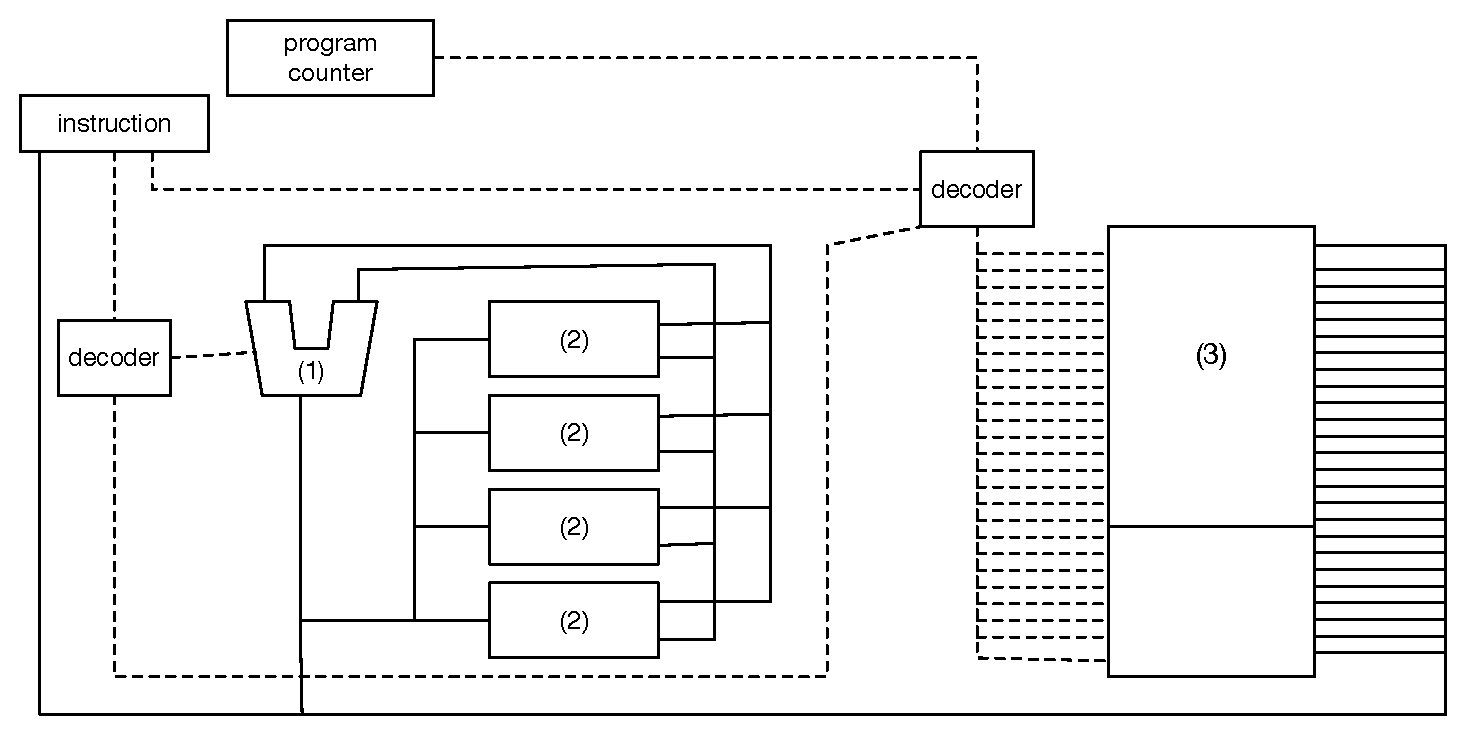
\includegraphics[scale=0.5]{./Figure/elementaryCS-figCPU-exam.eps}
  \end{center}

\paragraphskip
\nitem{\bf 問10.}(配点 15 点)\\
次に示したのは言語 Ruby で書かれたプログラムである.
このプログラムについて以下の問いに答えよ.

\begin{verbatim}
CODE_a = 97
CODE_z = 122
ALPHABET_SIZE =26

def letter2index (letter)
  return (letter - CODE_a)
end
def index2letter (index)
  return (index + CODE_a)
end
def transform(char,key)
  index = letter2index(char)
  c_index = (index + (letter2index(key))) % ALPHABET_SIZE
  return(index2letter(c_index))
end
def vigenere (key,message,chipher_text)
  key_length=key.length
  message_length=message.length
  for i in 0..(message_length-1)
    if CODE_a <= message[i] && message[i] <= CODE_z
       chipher_text[i] = transform(message[i],key[i % key_length])
    else
       chipher_text[i] = message[i]
    end
  end
end
def encipher(key, message)
  letters = message.unpack("C*")
  keys = key.unpack("C*")
  chipher_letters = Array.new(message.length)
  vigenere(keys,letters,chipher_letters)
  return (chipher_letters.pack("C*"))
end

hirabun = gets.chomp
angobun = encipher("vigenere", hirabun)
puts(angobun)
\end{verbatim}

\nitem{(1)}
平文 "hello" が入力として与えられたときの暗号文を示せ.
\nitem{(2)}
文字の置き換えをどのようにしているか modulo の計算式を示しながら説明せよ.

\end{document}
